\documentclass[10pt]{article}

\usepackage[margin=0.72in]{geometry}
\usepackage{amsmath}
\usepackage{amssymb}
\usepackage{booktabs}
\usepackage{graphicx}
\usepackage{hyperref}
\usepackage{enumitem}
\usepackage{caption}
\usepackage{cite}
\usepackage{float}
\usepackage{placeins}

\hypersetup{
  colorlinks=true,
  linkcolor=black,
  citecolor=black,
  urlcolor=blue
}

\setlist[itemize]{leftmargin=1.15em, itemsep=0.1em, topsep=0.1em}
\setlength{\parindent}{0pt}
\setlength{\parskip}{0.28em}
\captionsetup{font=small}

\title{Dynamic Regime Adapter for Zero-Gradient Time-Series Test-Time Adaptation}
\author{Lu Anhe 1235055 \\ Wei Lai 1306065 \\ Xu Fei 1308365}
\date{}

\begin{document}
\maketitle

\begin{abstract}
We study whether a time-series test-time adapter can be learned before deployment and then applied without online backpropagation. Our main method, the Dynamic Regime Adapter, uses a lightweight RegimeEncoder to infer a latent context factor from recent history and a GateGenerator to produce horizon-wise forecast corrections. The adapter is trained offline while the forecasting backbone remains frozen, and test-time inference requires only a single forward pass. On Weather/DLinear/96 it achieves the best clean-test MSE improvement among the compared methods, and on ETTh1/DLinear/96 it slightly outperforms online COSA variants in MSE while avoiding test-time gradient updates. Under ETTh1/DLinear/horizon-720 black-swan shifts, the meta-trained adapter also achieves the lowest post-shift MSE on level, trend, and spike shifts, while COSA+ remains best on variance shift. We also include COSA+ as an online COSA-family ablation: it is useful for diagnosing long-horizon robustness, but it is treated as supporting evidence rather than the central contribution.
\end{abstract}

\section{Introduction}
Time-series forecasting models are usually evaluated on fixed train, validation, and test splits, but deployed streams often shift because of sensor faults, weather anomalies, demand spikes, or structural changes. Test-time adaptation addresses this mismatch by correcting predictions during deployment. COSA adapts forecasts through a lightweight output-space module, but it still requires gradient-based online optimization during evaluation.

This project focuses on a different operating point: learning the adaptation rule offline, then applying it at test time without backpropagation. The proposed Dynamic Regime Adapter treats recent context as evidence for a latent regime. A RegimeEncoder extracts a low-dimensional factor $z$, and a GateGenerator maps $z$ to a horizon-wise correction gate. Because the backbone is frozen and the adapter is evaluated under \texttt{torch.no\_grad()}, deployment only adds a small forward pass.

We compare the adapter against the frozen DLinear backbone and online COSA variants on Weather and ETTh1. The main empirical result is that the Dynamic Regime Adapter can improve clean-test MSE with no inference-time gradient updates. COSA+ is included as a supporting online ablation to understand how vector gates behave under abrupt long-horizon shifts; those experiments help contextualize the cost--accuracy trade-off but are not presented as the main method.

\section{Related Work}
\textbf{Time-series forecasting and zero-shot adaptation.} Long-horizon forecasting has been studied with linear models, recurrent models, convolutional models, and Transformer-based architectures. DLinear \cite{zeng2023dlinear} is a simple but competitive baseline that decomposes time series and applies linear forecasting layers. Meta-learning work on zero-shot forecasting shows that forecasting models can learn transferable adaptation mechanisms across time series without retraining on each target dataset \cite{oreshkin2021meta}. This motivates our design choice: adaptation behavior can be learned before deployment rather than relying entirely on online gradient updates.

\textbf{Test-time adaptation.} Test-time adaptation methods update either model parameters, normalization statistics, or lightweight auxiliary modules during inference. COSA is the closest related method because it keeps the forecasting backbone mostly frozen and corrects forecasts through a context-aware output-space adapter \cite{cosa2026}. However, COSA still updates adapter parameters online during test-time evaluation. Meta-TTT studies a meta-learning minimax formulation for test-time training and highlights the value of learning adaptation objectives before deployment \cite{tao2025metattt}. Recent time-series TTA work further shows that lightweight adaptation can help under non-stationarity, but aggressive online updates can be unstable under noisy streams or financial regimes \cite{wu2026tta}. Our Dynamic Regime Adapter therefore targets a conservative zero-gradient inference setting: it trades some online flexibility for lower deployment cost and more predictable inference.

\textbf{Regime learning under distribution shift.} Many practical time-series domains contain latent regimes, such as stable periods, high-volatility periods, structural level changes, and local shocks. Regime-aware financial forecasting methods such as RAM-Net use meta-learning to re-weight samples under changing market conditions \cite{jang2025ramnet}. In contrast, our method uses recent context to infer a latent regime factor and generate horizon-wise correction gates. The latent representation $z$ is not used as a hard regime label; it is a continuous correction signal that can be inspected after training.

\section{Method}
\subsection{Problem Formulation}
Let $X \in \mathbb{R}^{B \times L \times C}$ be a historical context window with batch size $B$, context length $L$, and $C$ variables. A frozen forecasting backbone produces a base prediction
\begin{equation}
  H=f_{\theta}(X) \in \mathbb{R}^{B \times T \times C},
\end{equation}
where $T$ is the forecast horizon and $\theta$ remains fixed during adaptation. The shared goal of COSA+, original COSA, and the Dynamic Regime Adapter is to construct an adapted forecast $\hat{Y}$ from $(H,X)$ without retraining the backbone. The key difference is where adaptation is learned: COSA-style methods optimize a lightweight output adapter online during test-time evaluation, while the Dynamic Regime Adapter learns a reusable mapping offline and applies it by a single forward pass.


\subsection{Dynamic Regime Adapter}
The Dynamic Regime Adapter contains a RegimeEncoder and a GateGenerator. Given context window $X \in \mathbb{R}^{B \times L \times C}$ and frozen forecast $H=f_\theta(X)$, the RegimeEncoder maps context to a latent factor
\begin{equation}
  z = E_{\phi}(X), \qquad z \in \mathbb{R}^{B \times d}.
\end{equation}
The GateGenerator then outputs a horizon-wise correction gate
\begin{equation}
  g = G_{\phi}(z), \qquad g \in \mathbb{R}^{B \times T},
\end{equation}
and the corrected forecast is
\begin{equation}
  \hat{Y}=H+\tanh(g)[:,:, \mathrm{None}] \odot H.
\end{equation}

The RegimeEncoder is a lightweight one-dimensional temporal CNN with ReLU activations, dropout, adaptive average pooling, and a final linear projection. The GateGenerator is a two-layer MLP. The hyperbolic tangent bounds the correction magnitude, and the final gate layer is initialized near zero so the adapter initially behaves close to the identity mapping. During offline meta-training, the frozen backbone first constructs tuples $(X,H,Y)$ on validation batches, then only the adapter parameters are updated. We use either pure MSE or a mixed loss,
\begin{equation}
  \mathcal{L}=0.7\,\mathrm{MSE}(\hat{Y},Y)+0.3\,\mathrm{MAE}(\hat{Y},Y).
\end{equation}
At test time, inference is wrapped in \texttt{torch.no\_grad()}, so no online backpropagation is performed.

\subsection{Online COSA Baselines}
COSA uses a frozen forecasting backbone and adapts a small output-space module online at test time \cite{cosa2026}. Given recent context $C_t$, a base forecast $\hat{Y}^{(0)}_t$, and adapter correction $H_t = W X_t^{(a)} + b$, original COSA produces
\begin{equation}
  \hat{Y}_t = \hat{Y}^{(0)}_t + \tanh(g) H_t,
\end{equation}
where $g \in \mathbb{R}$ is a scalar gate and $X_t^{(a)}=[\hat{Y}^{(0)}_t \| C_t]$ is the adapter input.

We use COSA and COSA+ as online baselines. COSA+ is not the main proposed method; it is an ablation of the online adapter design that helps quantify what can be recovered when test-time gradients are allowed. COSA+ combines a horizon-wise vector gate with richer context statistics. The vector gate replaces scalar $g$ with
\begin{equation}
  g \in \mathbb{R}^{L}, \qquad \alpha=\tanh(g)\in\mathbb{R}^{L},
\end{equation}
and applies $\alpha$ element-wise across prediction steps:
\begin{equation}
  \hat{Y}_{t,\ell} = \hat{Y}^{(0)}_{t,\ell} + \alpha_{\ell} H_{t,\ell}.
\end{equation}
The richer context replaces mean-only history $C_t=[\mu_{t-K},\ldots,\mu_{t-1}]$ with mean-plus-standard-deviation history
\begin{equation}
  C_t=[\mu_{t-K},\sigma_{t-K},\ldots,\mu_{t-1},\sigma_{t-1}] \in \mathbb{R}^{2K}.
\end{equation}
\subsection{Black-Swan Shift Protocol}
To stress-test robustness, we transform the second part of a test stream after a shift point $T_{\mathrm{shift}}$:
\begin{equation}
  x'_t =
  \begin{cases}
    x_t, & t<T_{\mathrm{shift}}, \\
    S(x_t;\alpha), & t\geq T_{\mathrm{shift}},
  \end{cases}
\end{equation}
where $\alpha$ is the shift magnitude, $\sigma_{\mathrm{tr}}$ is the training-set standard deviation, and $\mu_{\mathrm{pre}}$ is the pre-shift mean. Table~\ref{tab:shift-defs} summarizes the four synthetic shifts. We report \texttt{mse\_after\_50}, which ignores the first 50 post-shift steps and therefore emphasizes recovery after the boundary rather than only the immediate discontinuity.

\begin{table}[H]
\centering
\small
\caption{Synthetic black-swan shift definitions.}
\label{tab:shift-defs}
\begin{tabular}{lll}
\toprule
Shift type & Transformation after $T_{\mathrm{shift}}$ & Intuition \\
\midrule
Level & $x'_t=x_t+\alpha\sigma_{\mathrm{tr}}$ & sudden mean change \\
Variance & $x'_t=\mu_{\mathrm{pre}}+\alpha(x_t-\mu_{\mathrm{pre}})$ & volatility scaling \\
Trend & $x'_t=x_t+(t-T_{\mathrm{shift}})\alpha\sigma_{\mathrm{tr}}/100$ & gradual drift \\
Spike & $x'_{T_{\mathrm{shift}}}=x_{T_{\mathrm{shift}}}+\alpha\sigma_{\mathrm{tr}}$ & single extreme disturbance \\
\bottomrule
\end{tabular}
\end{table}

\section{Experimental Setup}
We evaluate DLinear on Weather and ETTh1. Weather has 21 variables, ETTh1 has 7 variables, and the DLinear backbone is frozen throughout. Each dataset starts from a single chronological time-series file; the code constructs standard train, validation, and test splits from that sequence rather than using separate validation files. The backbone is trained on the training split, the Dynamic Regime Adapter is meta-trained on validation batches with simulated context shifts, and final performance is evaluated on the held-out test split. Prediction lengths are 96 and 720. Compared methods include the frozen backbone, original COSA, COSA+, and Dynamic Regime Adapter variants: untrained, pure MSE, and mixed loss. The Dynamic Regime Adapter uses latent dimension 16, hidden dimension 64, dropout 0.1, learning rate 0.001, batch size 64, and 10 meta-training epochs. The Weather/96 mixed-loss run uses 81 validation meta-training batches.

\begin{table}[h]
\centering
\small
\caption{Experimental settings.}
\label{tab:settings}
\begin{tabular}{ll}
\toprule
Setting & Value \\
\midrule
Datasets & Weather, ETTh1 \\
Backbone & Frozen DLinear \\
Prediction lengths & 96, 720 \\
Black Swan shifts & Level, Variance, Trend, Spike \\
Black-swan metric & \texttt{mse\_after\_50} for shifted-data evaluation \\
Weather/96 COSA setting & batch size 64, $S=3$, $K=10$, PAAS disabled \\
ETTh1 COSA setting & default batch size 48, $S=3$, $K=10$, PAAS disabled \\
\bottomrule
\end{tabular}
\end{table}


\section{Results}
\subsection{Adapter Meta-Training Behavior}
The mixed-loss Dynamic Regime Adapter starts close to identity, as intended: before meta-training, Weather validation MSE is 0.481351 for the frozen backbone and 0.481352 for the adapter. After 10 epochs, adapter validation MSE drops to 0.432192, while the recorded training objective decreases from 0.427963 in epoch 1 to 0.399003 in epoch 10. This supports the interpretation that the adapter is learning a reusable correction rule rather than exploiting random initialization; the untrained test result in Table~\ref{tab:weather-clean} further confirms this identity behavior.

\subsection{Clean-Test Performance}
Table~\ref{tab:weather-clean} shows that on Weather/96, the mixed-loss Dynamic Regime Adapter achieves the best MSE improvement (+2.48\%) while requiring no test-time gradient updates. Its MAE is worse than online COSA variants, so the result should be interpreted as an MSE-focused gain rather than a uniform improvement across metrics. Table~\ref{tab:etth1-clean} extends evaluation to ETTh1. At horizon 96, Dynamic meta-trained achieves the best MSE improvement (+1.58\%) with nearly unchanged MAE. At horizon 720, online COSA+ gives the strongest numbers, while Dynamic meta-trained still improves MSE by +3.59\% and MAE by +1.46\% without online optimization. These results support the adapter's main value proposition: competitive clean-test correction with lower deployment complexity.

\begin{table}[H]
\centering
\small
\caption{Test performance on Weather/DLinear/96. Dynamic Regime Adapter variants use zero-gradient inference; COSA variants require online test-time backpropagation.}
\label{tab:weather-clean}
\begin{tabular}{lrrrr}
\toprule
Method & MSE & MAE & MSE Impr. & MAE Impr. \\
\midrule
Frozen backbone & 0.195218 & 0.234493 & 0.00\% & 0.00\% \\
Dynamic untrained & 0.195219 & 0.234494 & -0.00\% & -0.00\% \\
Dynamic pure MSE & 0.191855 & 0.243863 & +1.72\% & -4.00\% \\
Dynamic mixed loss & \textbf{0.190373} & 0.240629 & \textbf{+2.48\%} & -2.62\% \\
COSA original & 0.191272 & \textbf{0.237397} & +2.02\% & -1.24\% \\
COSA+ & 0.191641 & 0.237735 & +1.83\% & -1.38\% \\
\bottomrule
\end{tabular}
\end{table}

\begin{table}[!htbp]
\centering
\small
\caption{Test performance on ETTh1/DLinear at horizons 96 and 720. Dynamic Regime Adapter uses zero-gradient inference; COSA variants use online test-time optimization.}
\label{tab:etth1-clean}
\begin{tabular}{rlrrrr}
\toprule
Horizon & Method & MSE & MAE & MSE Impr. & MAE Impr. \\
\midrule
96 & Frozen backbone & 0.459481 & 0.456869 & 0.00\% & 0.00\% \\
96 & Dynamic untrained & 0.459479 & 0.456868 & $\sim$0.00\% & $\sim$0.00\% \\
96 & Dynamic meta-train & \textbf{0.452199} & 0.456842 & \textbf{+1.58\%} & +0.01\% \\
96 & COSA original & 0.452734 & \textbf{0.452890} & +1.47\% & \textbf{+0.87\%} \\
96 & COSA+ & 0.453148 & 0.453327 & +1.38\% & +0.77\% \\
720 & Frozen backbone & 0.705116 & 0.611058 & 0.00\% & 0.00\% \\
720 & Dynamic untrained & 0.705116 & 0.611058 & $\sim$0.00\% & $\sim$0.00\% \\
720 & Dynamic meta-train & 0.679836 & 0.602107 & +3.59\% & +1.46\% \\
720 & COSA original & 0.673144 & 0.600635 & +4.53\% & +1.70\% \\
720 & COSA+ & \textbf{0.670793} & \textbf{0.599874} & \textbf{+4.86\%} & \textbf{+1.83\%} \\
\bottomrule
\end{tabular}
\end{table}

\FloatBarrier
\subsection{Black-Swan Shifted Data Performance}
Table~\ref{tab:dynamic_blackswan_etth1_h720} reports the black-swan shifted-data comparison on ETTh1/DLinear/h=720. Beyond clean-test evaluation, we further test whether the Dynamic Regime Adapter can transfer to black-swan shifted data.

The untrained dynamic adapter is almost identical to No TTA, which confirms that the improvement does not come from random initialization. After offline meta-training, the Dynamic Regime Adapter achieves the lowest post-shift MSE on level, trend, and spike shifts, while COSA+ remains slightly strongest on the variance shift. This suggests that the offline meta-training learns a correction signal that transfers beyond clean-test conditions to several synthetic abrupt shifts in ETTh1/horizon-720. The result strengthens the complementary narrative: COSA+ provides strong online adaptation through test-time gradient updates, while the Dynamic Regime Adapter can deliver competitive or better post-shift recovery without online backpropagation.

\begin{table}[H]
\centering
\small
\caption{Dynamic Regime Adapter black-swan shifted-data comparison on ETTh1/DLinear/h=720, shift magnitude 3.0. Metric is \texttt{mse\_after\_50}. Lower is better.}
\label{tab:dynamic_blackswan_etth1_h720}
\resizebox{\linewidth}{!}{%
\begin{tabular}{lrrrrr}
\toprule
Shift type & No TTA & Dynamic untrained & COSA original & COSA+ & Dynamic meta-trained \\
\midrule
Level & 1.514135 & 1.514134 & 1.390041 & 1.370746 & \textbf{1.350300} \\
Variance & 1.401813 & 1.401811 & 1.312613 & \textbf{1.303288} & 1.305544 \\
Trend & 1.092508 & 1.092506 & 0.996507 & 0.985433 & \textbf{0.972506} \\
Spike & 1.071504 & 1.071502 & 0.979771 & 0.969925 & \textbf{0.957617} \\
\bottomrule
\end{tabular}%
}
\end{table}

\subsection{Latent Regime Visualization}
Figure~\ref{fig:latent-tsne} shows t-SNE projections of latent factors $z$ after adapter meta-training. Weather/DLinear/96 does not form clean regime clusters, while ETTh1/DLinear/720 shows stronger local structure with several curved trajectories. We therefore interpret $z$ as a continuous correction signal rather than a discrete regime classifier. This is consistent with the adapter design: the latent factor is used to generate soft gates, not to assign hard regime labels.

\begin{figure}[!htbp]
\centering
\begin{minipage}{0.48\linewidth}
\centering
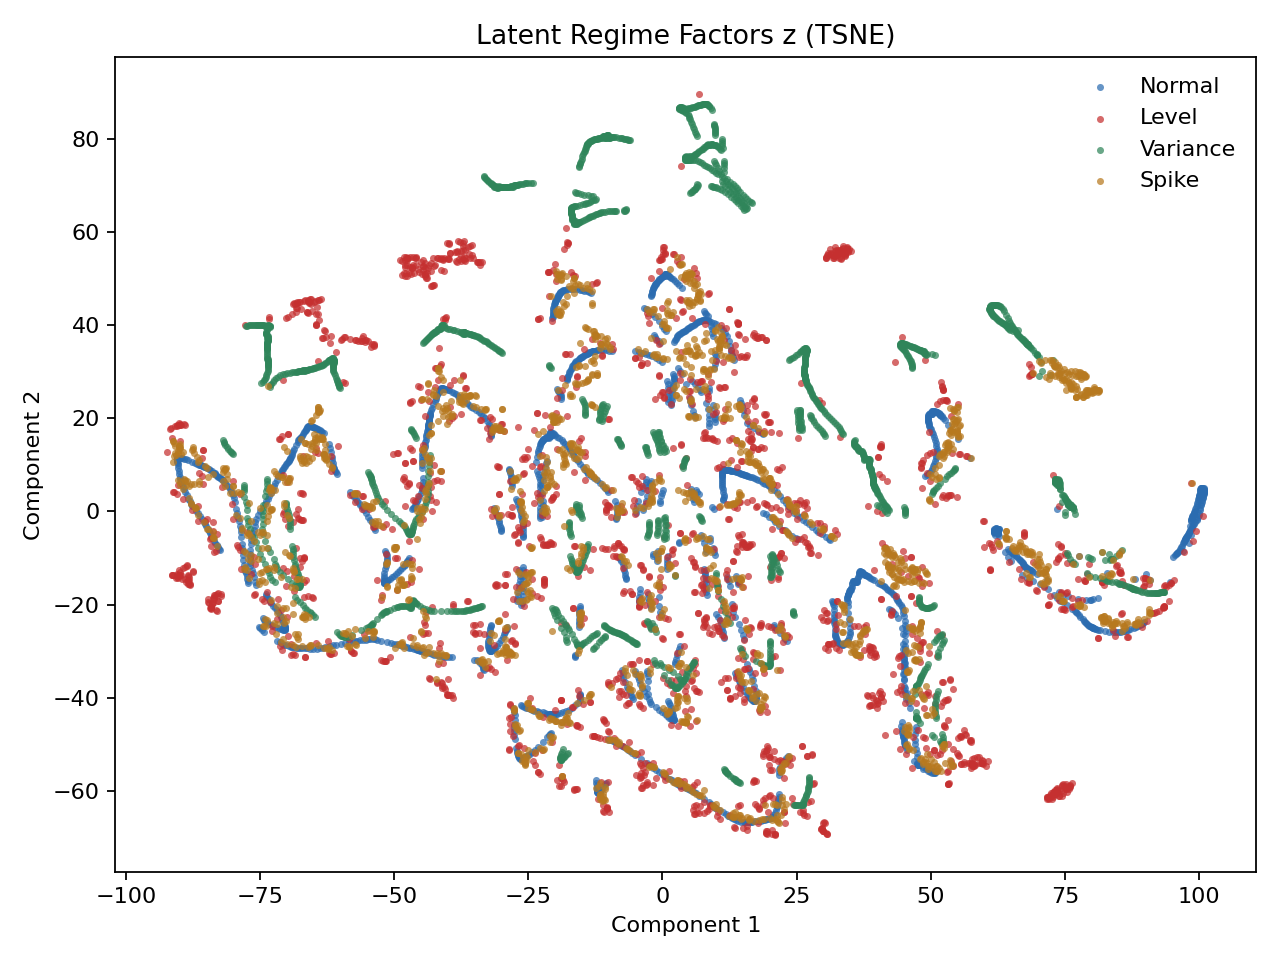
\includegraphics[width=\linewidth]{../results/regime_adapter_latents_mixed_loss/tsne/DLinear/weather/96/latent_regimes.png}
\caption*{Weather/DLinear/96}
\end{minipage}\hfill
\begin{minipage}{0.48\linewidth}
\centering
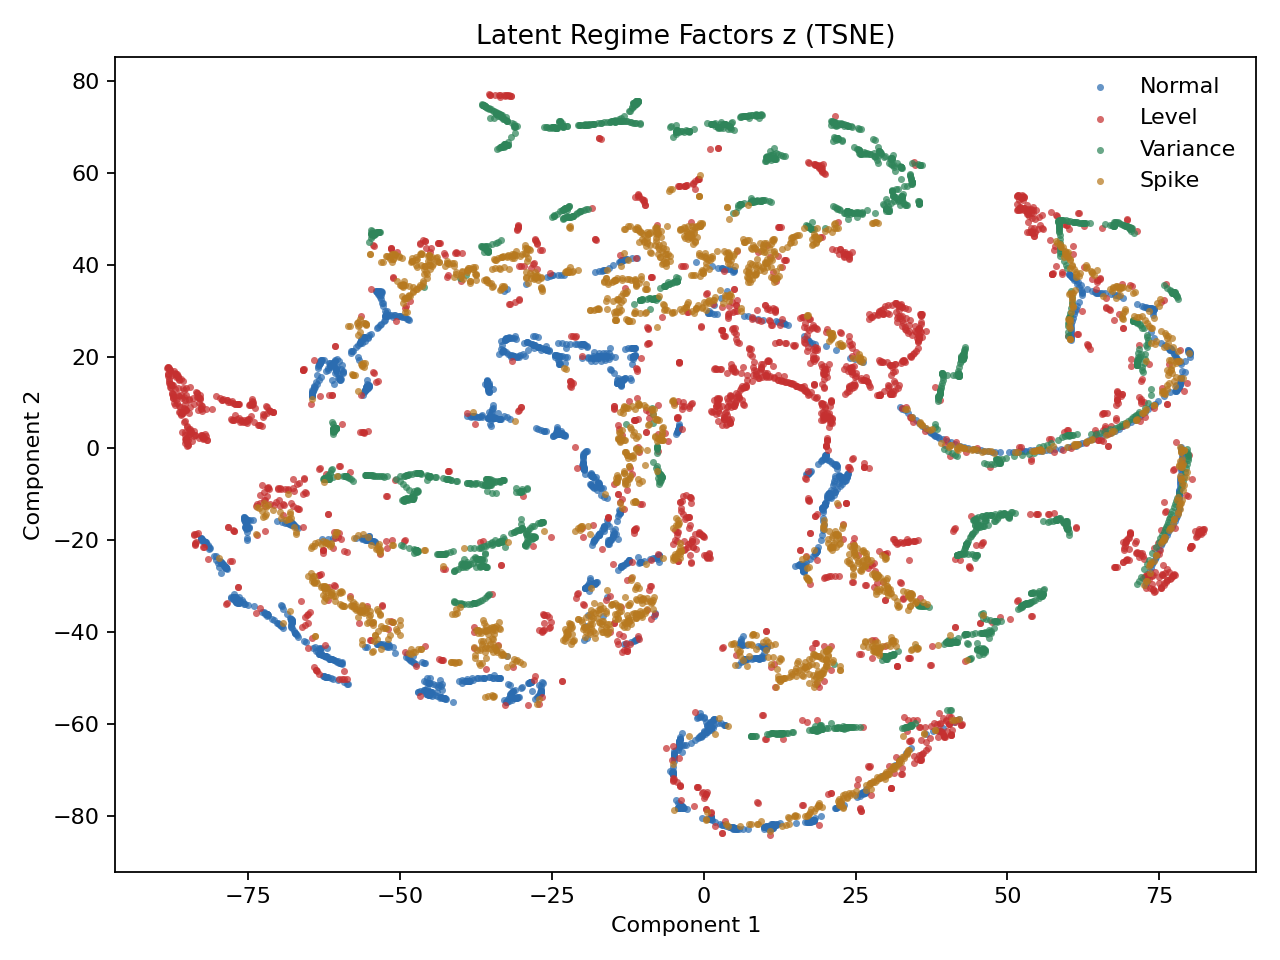
\includegraphics[width=\linewidth]{../results/regime_adapter_latents_etth1_720/tsne/DLinear/ETTh1/720/latent_regimes.png}
\caption*{ETTh1/DLinear/720}
\end{minipage}
\caption{t-SNE projections of Dynamic Regime Adapter latent factors $z$. The structure is continuous rather than a clean discrete taxonomy.}
\label{fig:latent-tsne}
\end{figure}

\FloatBarrier
\subsection{Additional Weather Robustness Check}
Weather gives a more cautious additional robustness result. Table~\ref{tab:weather-blackswan} shows that online adaptation clearly helps under Weather horizon-720 shifts, but full COSA+ is slightly worse than original COSA on most shift types. This prevents overclaiming: richer online gates are not a free improvement, especially when the adaptation signal is spread across more variables.

\begin{table}[!htbp]
\centering
\small
\caption{Weather/DLinear/horizon-720 black-swan \texttt{mse\_after\_50}. Lower is better.}
\label{tab:weather-blackswan}
\begin{tabular}{lrrrr}
\toprule
Shift type & No TTA & COSA original & RichCtx & COSA+ \\
\midrule
Level & 0.534032 & \textbf{0.463273} & 0.463380 & 0.466465 \\
Variance & 0.224444 & 0.206461 & \textbf{0.206165} & 0.206648 \\
Trend & 0.206529 & \textbf{0.161436} & 0.161447 & 0.162618 \\
Spike & 0.202111 & 0.160640 & \textbf{0.160636} & 0.161715 \\
\bottomrule
\end{tabular}
\end{table}

\FloatBarrier

\section{Discussion}
The central trade-off is between online adaptability and deployment simplicity. Dynamic Regime Adapter moves adaptation into offline meta-training and then performs one zero-gradient correction pass at test time. This makes it attractive when inference latency, memory use, or deployment complexity matters. The clean-test results show that this simpler deployment path can still recover meaningful MSE gains on Weather and ETTh1.

The adapter is not uniformly better across metrics. On Weather/96, the mixed-loss adapter gives the best MSE but still has worse MAE than online COSA variants, showing that squared-error correction and absolute-error robustness are not identical. The latent visualizations also suggest that the learned factor $z$ should be treated as a continuous correction signal rather than a hard regime label. This is useful for the proposed gate-generation mechanism, but it does not by itself prove discrete regime discovery.

The black-swan experiments refine the cost of removing online gradients. COSA+ is a strong online robustness reference and remains best on ETTh1 variance shift, but the meta-trained Dynamic Regime Adapter is best on level, trend, and spike shifts without online optimization. Weather horizon-720 still prevents overclaiming: richer vector gates are not consistently better when the adaptation signal is noisier or distributed across more variables. The main conclusion is therefore not that either approach dominates, but that Dynamic Regime Adapter offers a practical zero-gradient alternative that can remain competitive under abrupt shifts.

The Dynamic Regime Adapter black-swan result is currently limited to ETTh1/DLinear/horizon-720 at one shift magnitude. Future work should test more datasets, horizons, and shift severities. Future work should also add quantitative latent-space diagnostics, such as silhouette score or neighborhood consistency, and tune the loss or gate regularization to reduce the Weather/96 MAE degradation.

\section{Conclusion}
We presented Dynamic Regime Adapter as an offline-learned, zero-gradient test-time adaptation module for time-series forecasting. By encoding recent context into a latent factor and generating horizon-wise correction gates, it improves clean-test MSE and remains competitive under ETTh1 black-swan shifted data while avoiding inference-time backpropagation. COSA+ is useful as an online robustness reference, especially for long-horizon abrupt shifts, but the main project contribution is the Dynamic Regime Adapter's lower-cost adaptation path.

\section*{AI Usage Statement}
AI tools were used to inspect code, organize experiments, debug scripts, and assist with report preparation. The reported experimental numbers are taken from the project result files generated by the authors' scripts.


\appendix
\section{Reproducibility Notes}
Experiments were run with the local COSA codebase using Python 3.10, PyTorch, NumPy, and SciPy. Final tables and figures are stored under \path{results/final_figures/}; Dynamic Regime Adapter checkpoints and latent visualizations are stored under the corresponding \path{results/regime_adapter*/} result directories.

\begin{thebibliography}{9}
\bibitem{zeng2023dlinear}
Ailing Zeng, Muxi Chen, Lei Zhang, and Qiang Xu. Are Transformers Effective for Time Series Forecasting? \textit{Proceedings of the AAAI Conference on Artificial Intelligence}, 2023.

\bibitem{cosa2026}
J. Im and H.-Y. Kwon. COSA: Context-aware output-space adapter for test-time adaptation in time series forecasting. \textit{International Conference on Learning Representations (ICLR)}, 2026.

\bibitem{oreshkin2021meta}
Boris N. Oreshkin, Dmitri Carpov, Nicolas Chapados, and Yoshua Bengio. Meta-learning framework with applications to zero-shot time-series forecasting. \textit{Proceedings of the AAAI Conference on Artificial Intelligence}, 2021. \url{https://arxiv.org/pdf/2002.02887}

\bibitem{jang2025ramnet}
J. Jang, T. Kim, D. Oh, and S.-H. Park. Adaptive sample weighting with regime-aware meta-learning framework for financial forecasting. In \textit{Proceedings of the 6th ACM International Conference on AI in Finance (ICAIF '25)}, ACM, 2025. \url{https://doi.org/10.1145/3768292.3770374}

\bibitem{tao2025metattt}
Chen Tao, Li Shen, and Soumik Mondal. Meta-TTT: A meta-learning minimax framework for test-time training. \textit{International Conference on Machine Learning and Applications (ICMLA)}, 2025. \url{https://doi.org/10.1109/ICMLA66185.2025.00008}

\bibitem{wu2026tta}
Yurui Wu, Qingying Deng, Wonou Chung, and Mairui Li. Test-time adaptation for non-stationary time series: From synthetic regime shifts to financial markets, 2026. \url{https://arxiv.org/pdf/2602.00073}

\bibitem{cosa_repo}
BigBases. COSA\_ICLR2026: Official implementation of COSA. GitHub repository. \url{https://github.com/bigbases/COSA_ICLR2026}

\bibitem{wu2021autoformer}
Haixu Wu, Jiehui Xu, Jianmin Wang, and Mingsheng Long. Autoformer: Decomposition Transformers with Auto-Correlation for Long-Term Series Forecasting. \textit{NeurIPS}, 2021.

\bibitem{lai2018lstnet}
Guokun Lai, Wei-Cheng Chang, Yiming Yang, and Hanxiao Liu. Modeling Long- and Short-Term Temporal Patterns with Deep Neural Networks. \textit{SIGIR}, 2018.
\end{thebibliography}

\end{document}
